\subsection{Full NLO QCD corrections with \textbf{\texttt{ggxy}}}

%\textit{Authors:} Joshua Davies, Kay Sch\"onwald, Matthias Steinhauser, Daniel Stremmer

\textbf{Joshua Davies, Kay Schönwald, Matthias Steinhauser, Daniel Stremmer~\cite{Davies:2018qvx,Davies:2023vmj,Davies:2025qjr}.}

\noindent An alternative to the numerical approaches described in Sections~\ref{sec:fullPS} and~\ref{sec:nlo2} is to consider series
expansions of the two-loop virtual amplitude in complementary kinematic regions; here we consider in particular both the high-energy and forward-scattering regions.

The
``high-energy'' expansion has been considered in Ref.~\cite{Davies:2018qvx}, which assumes the
scale hierarchy $s,|t| > m_t^2 > m_h^2$ to produce a Taylor series in $m_h$ and a deep
asymptotic expansion in $m_t$. Pad\'e approximants are used to greatly increase
the region of validity of the expansion, ultimately producing a good description
of the amplitude for $p_T$ values above around 150 GeV. The high-energy expansion
also provides the input required by the resummation of \cite{Jaskiewicz:2024xkd}
(see Section~\ref{sec:scet}).
%
The small-$t$ expansion of \cite{Davies:2023vmj} also performs a Taylor expansion
in $m_h$, followed by an expansion in the forward limit, around $t=0$. This
produces a description for smaller $p_T$ values, below around 150 GeV, similar in
spirit to the small-$p_T$ expansion of \cite{Bonciani:2018omm}.

The combination of both regions
covers the whole phase space~\cite{Davies:2023vmj} and can
thus be used to compute the two-loop
virtual amplitude. The numerical evaluation
is
extremely fast and yet retains full dependence on the input parameters,
in particular the masses of the Higgs boson and top quark, and the ability to change
the top quark renormalization scheme and scale without expensive numerical integration.
The two-loop virtual amplitudes based on this approach are publicly available in the \texttt{C++}
library \texttt{ggxy}~\cite{Davies:2025qjr}, which is able to produce total cross sections and differential distributions in about 30 minutes on a laptop.

An example is shown in Table~\ref{tab::ggxy_kappa}, where we present the total cross sections at NLO QCD accuracy for various
values of $\kappa_\lambda \equiv \lambda_{hhh}/\lambda_{hhh}^{\rm SM}$. We show results for $\sqrt{s}=13$, $13.6$ and $14$~TeV,
and use both the on-shell and $\overline{\rm MS}$ top quark masses. Each value in Table~\ref{tab::ggxy_kappa} is obtained by averaging four seeds, each with a runtime of about $30$ minutes, yielding a total runtime of $72$ hours on a single core for the complete table.\footnote{Using the fact that the dependence on $\kappa_\lambda$ is quadratic would of course cut the runtime by half.}
\begin{table}[t!]
    \centering
    \renewcommand{\arraystretch}{1.2}
    \begin{tabular}{cc@{\hskip 7mm}lll}
%        \hline
        \toprule
         \multirow{2}{*}{$\kappa_\lambda$}&\multirow{2}{*}{Top quark mass scheme}
         & \multicolumn{3}{c}{$\sigma^{\rm NLO}_{\rm \tt ggxy}$ [fb]} \\
         \cmidrule(lr){3-5}
         & & $\sqrt{s}=13$~TeV & $\sqrt{s}=13.6$~TeV & $\sqrt{s}=14$~TeV\\
%        \hline\hline
        \midrule
        \multirow{2}{*}{$-5.0$} & on-shell & $ 511.7(4)^{+17.2\%}_{-14.4\%} $ & $ 564.0(4)^{+17.1\%}_{-14.3\%} $ & $ 599.3(5)^{+16.9\%}_{-14.1\%} $ \\
               & $\overline{\rm MS},\,\mu_t=m_{hh}/2$ & $ 521.8(4)^{+16.9\%}_{-14.2\%} $ & $ 574.3(4)^{+16.8\%}_{-14.0\%} $ & $ 609.8(5)^{+16.7\%}_{-13.9\%} $   \\ %\hline
        \midrule
        \multirow{2}{*}{$-0.6$} & on-shell & $ 90.80(7)^{+15.8\%}_{-13.8\%} $ & $ 100.27(7)^{+15.7\%}_{-13.6\%} $ & $ 106.88(8)^{+15.6\%}_{-13.5\%} $ \\
               & $\overline{\rm MS},\,\mu_t=m_{hh}/2$ & $ 89.51(7)^{+16.2\%}_{-13.9\%} $ & $ 98.85(7)^{+16.0\%}_{-13.7\%} $ & $ 105.15(8)^{+15.9\%}_{-13.6\%} $ \\ %\hline
        \midrule
        \multirow{2}{*}{$0.0$} & on-shell & $ 61.54(5)^{+15.3\%}_{-13.5\%} $ & $ 68.14(5)^{+15.2\%}_{-13.4\%} $ & $ 72.60(6)^{+15.0\%}_{-13.3\%} $  \\
              & $\overline{\rm MS},\,\mu_t=m_{hh}/2$ & $ 59.84(5)^{+15.9\%}_{-13.8\%} $ & $ 66.01(5)^{+15.8\%}_{-13.6\%} $ & $ 70.34(6)^{+15.7\%}_{-13.5\%} $ \\ %\hline
        \midrule
        \multirow{2}{*}{$1.0$} & on-shell & $ 27.80(3)^{+13.9\%}_{-12.9\%} $ & $ 30.85(3)^{+13.7\%}_{-12.7\%} $ & $ 32.93(3)^{+13.6\%}_{-12.6\%} $  \\
              & $\overline{\rm MS},\,\mu_t=m_{hh}/2$ & $ 25.91(2)^{+15.4\%}_{-13.6\%} $ & $ 28.65(3)^{+15.2\%}_{-13.5\%} $ & $ 30.59(3)^{+15.2\%}_{-13.4\%} $ \\ %\hline
        \midrule
        \multirow{2}{*}{$2.4$} & on-shell & $ 12.053(9)^{+14.8\%}_{-13.3\%} $ & $ 13.381(9)^{+14.7\%}_{-13.2\%} $ & $ 14.26(1)^{+14.6\%}_{-13.1\%} $  \\
              & $\overline{\rm MS},\,\mu_t=m_{hh}/2$ & $ 11.056(8)^{+17.6\%}_{-14.7\%} $ & $ 12.240(9)^{+17.4\%}_{-14.6\%} $ & $ 13.069(9)^{+17.3\%}_{-14.5\%} $  \\ %\hline
        \midrule
        \multirow{2}{*}{$5.0$} & on-shell & $ 80.38(6)^{+19.5\%}_{-15.4\%} $ & $ 88.14(6)^{+19.3\%}_{-15.3\%} $ & $ 93.60(7)^{+19.2\%}_{-15.2\%} $ \\
              & $\overline{\rm MS},\,\mu_t=m_{hh}/2$ & $ 84.67(6)^{+18.7\%}_{-15.0\%} $ & $ 92.93(7)^{+18.5\%}_{-14.9\%} $ & $ 98.69(7)^{+18.5\%}_{-14.8\%} $ \\
%        \noalign{\smallskip}\hline\noalign{\smallskip}
        \bottomrule
    \end{tabular}
    \caption{Total cross sections for $\sqrt{s}=13, 13.6, 14~\textup{TeV}$ in the on-shell and $\overline{\rm MS}$ top quark mass schemes. Results are obtained with $m_t=172.5$~GeV, $m_h=125~\textup{GeV}$ and $\mu_R=\mu_F=m_{hh}/2$ with the NLO NNPDF3.1 \cite{NNPDF:2017mvq} PDF set.}   \label{tab::ggxy_kappa}
\end{table}

\texttt{ggxy} has been linked to \texttt{Powheg}~\cite{Alioli:2010xd} (\texttt{ggxy\_ggHH}) to enable the matching to parton showers. Runtime tests have shown that
it is faster by a factor of $4$--$5$ than the previous implementation ({\tt ggHH}),
mainly due to the fast numerical evaluation of the one-loop $2\to 3$ processes for the real corrections with {\tt Recola}~\cite{Actis:2012qn,Actis:2016mpe}. Both \texttt{Powheg} implementations yield identical results for the fixed values of $m_t$ and $m_h$ in {\tt ggHH} as demonstrated in Fig.~\ref{fig::ggxy_nlo}, where we present the Higgs boson pair invariant mass distribution and the average Higgs boson transverse momentum distribution calculated with both tools without parton-shower effects. The lower panels display the $\sigma$ deviations with respect to the statistical uncertainties coming from the MC integration.

\begin{figure}[t]
  \begin{center}
  \begin{tabular}{cc}
     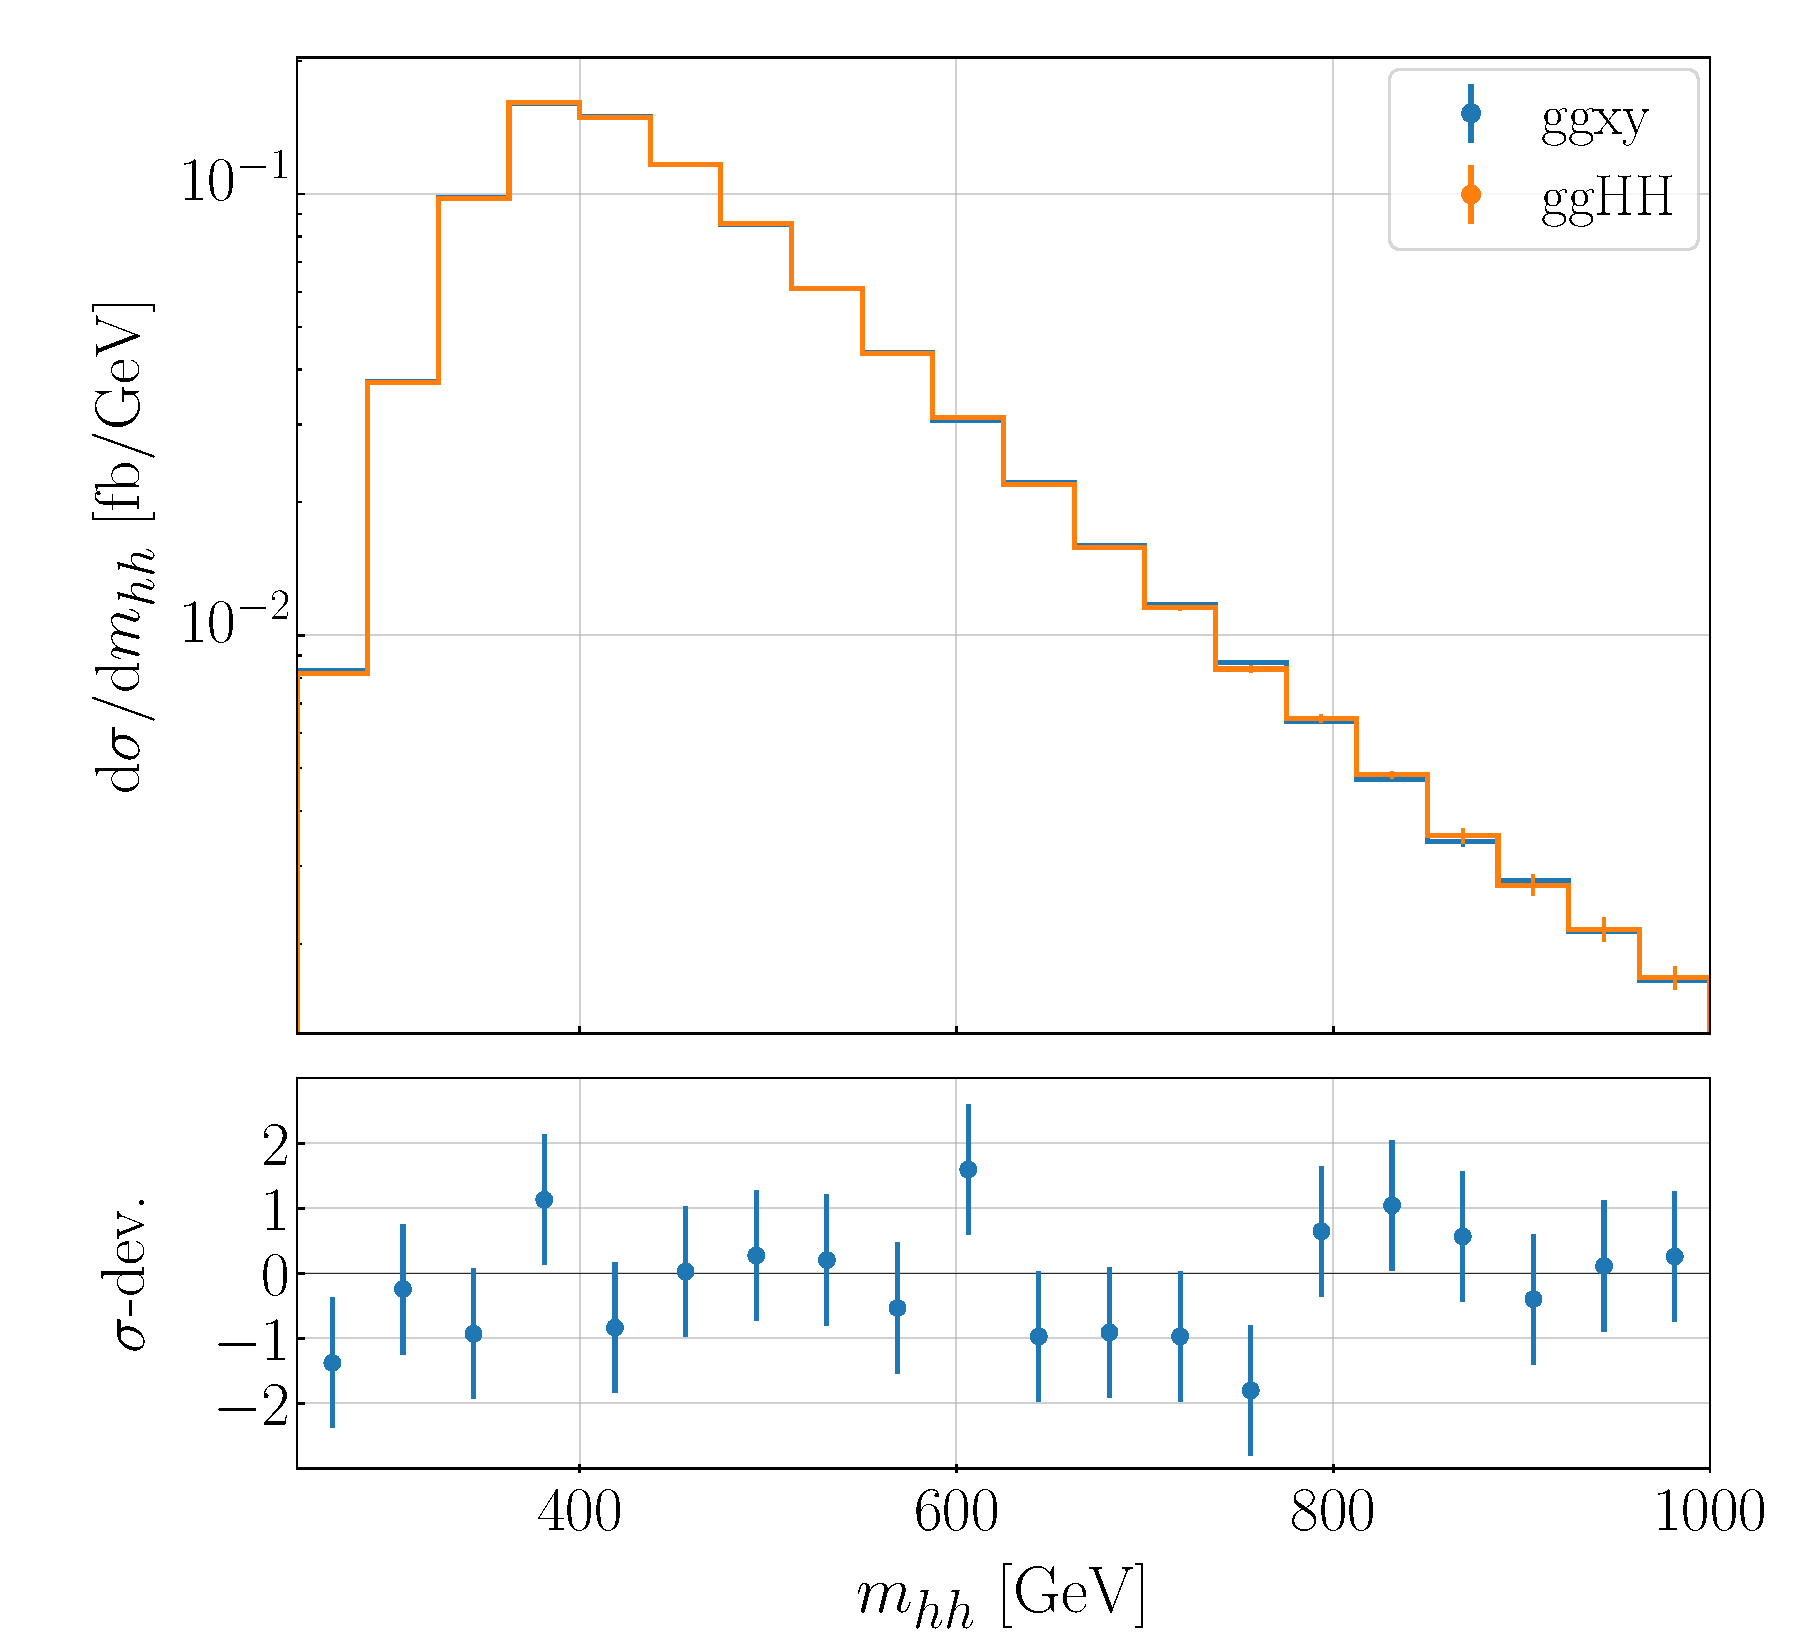
\includegraphics[width=0.45\textwidth]{NLO_QCD_SM/NLOggxy/Images/nlo_mhh_latexlabels.pdf}
     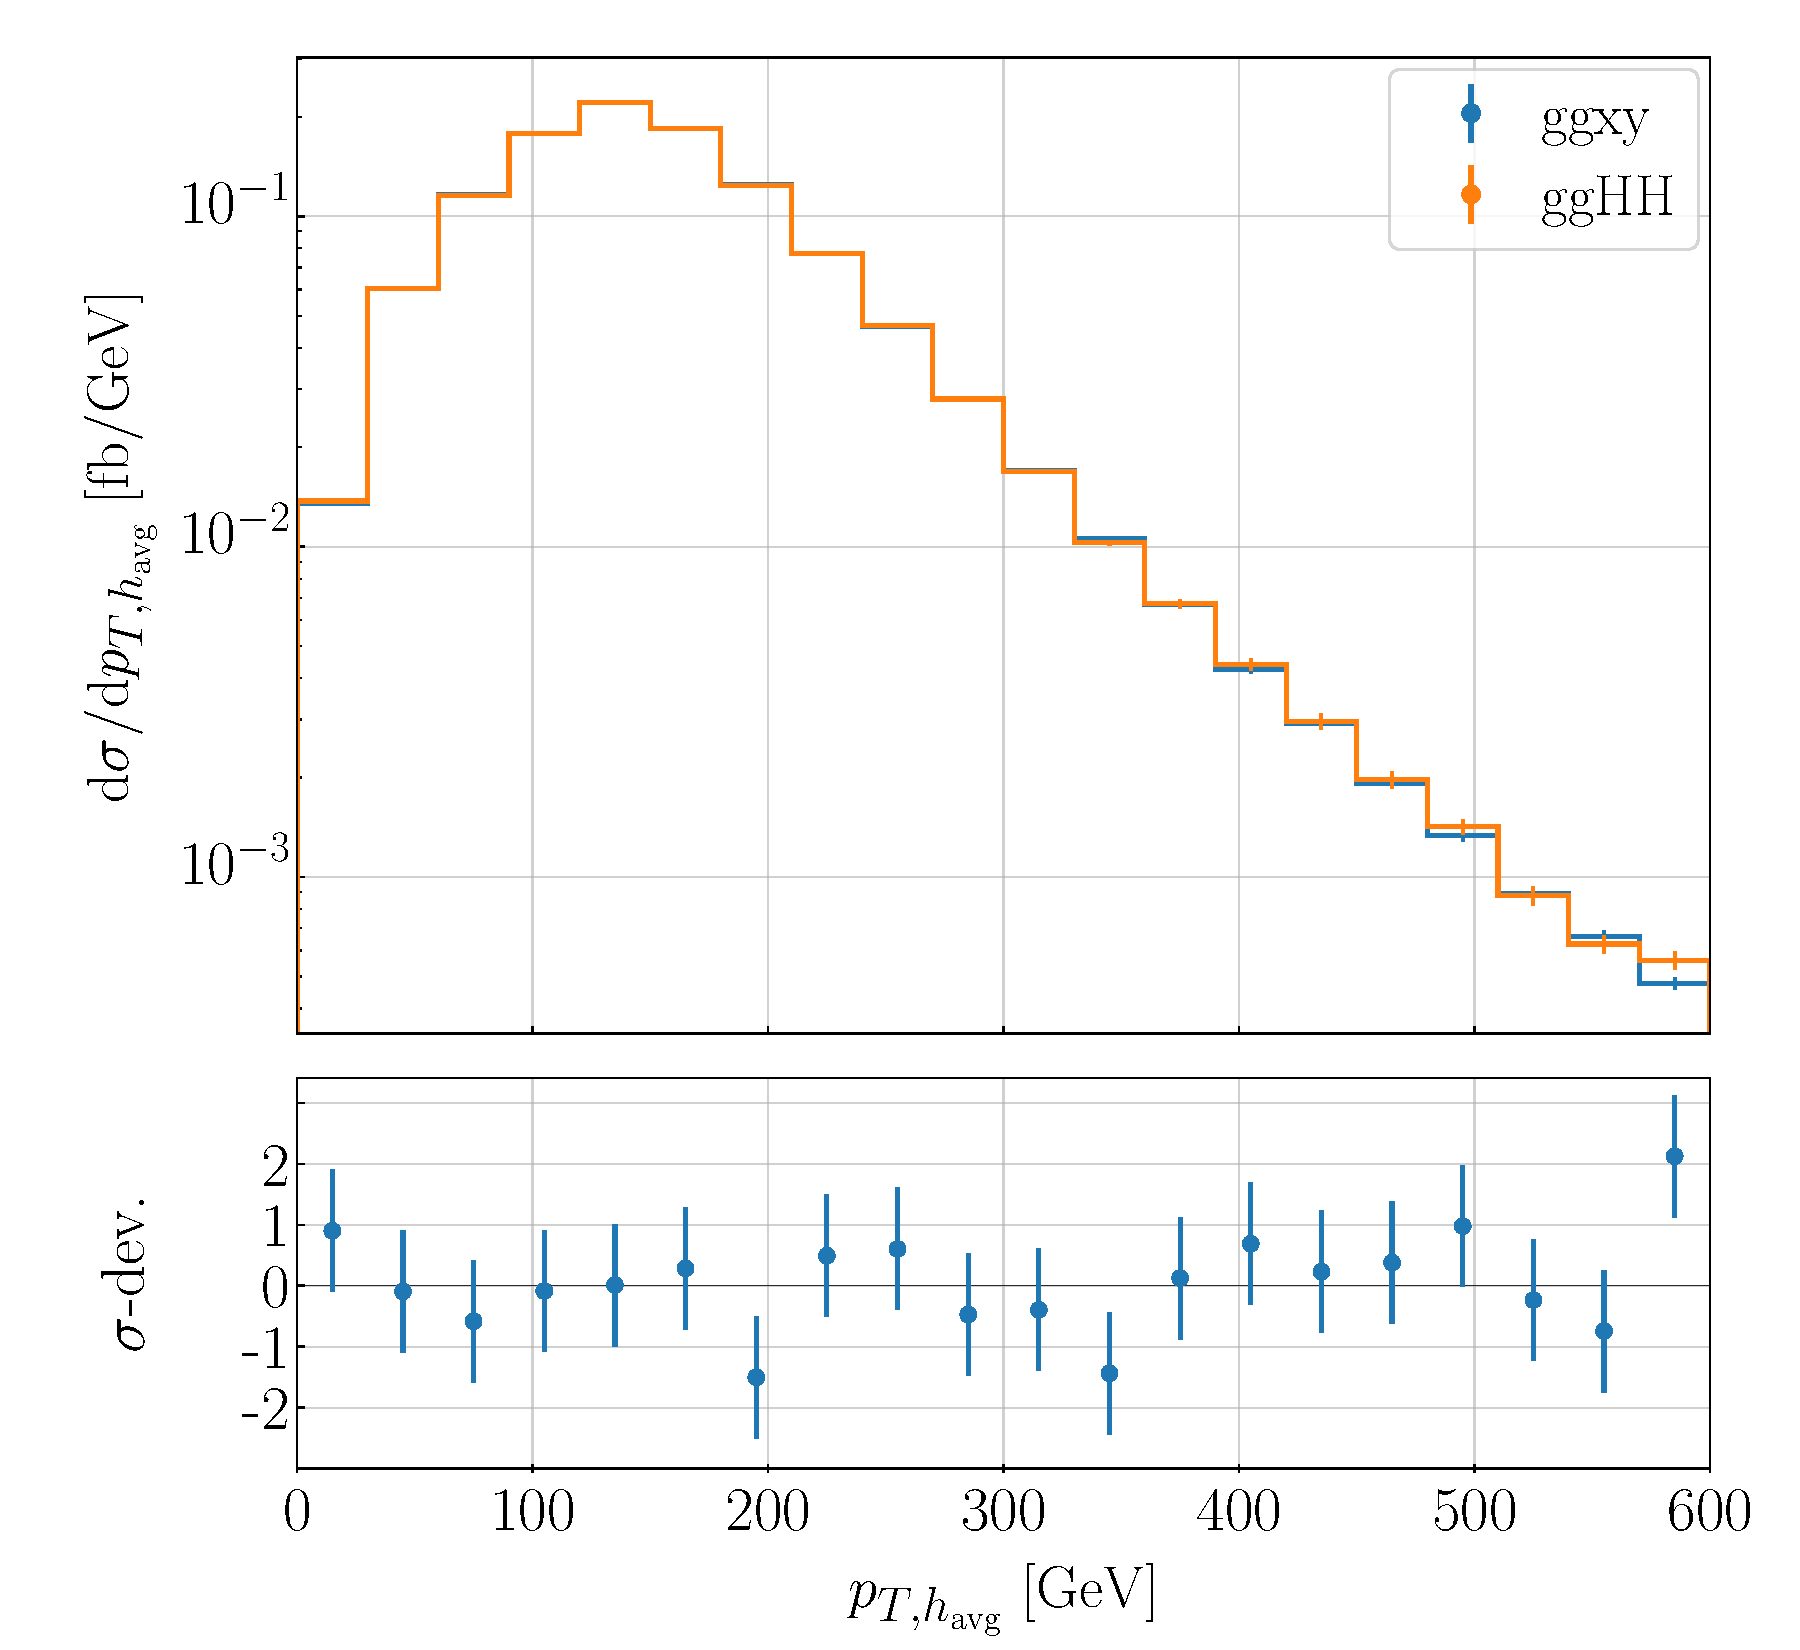
\includegraphics[width=0.45\textwidth]{NLO_QCD_SM/NLOggxy/Images/nlo_pthavg_latexlabels.pdf}
  \end{tabular}
  \end{center}
  \caption{\label{fig::ggxy_nlo} Comparison of
   NLO predictions generated with
   \texttt{ggxy\_ggHH} and \texttt{ggHH}
   for $m_{hh}$ and $p_{T,h_{\rm avg}}$ distributions for $\sqrt{s}=14~\textup{TeV}$. The lower panels display the $\sigma$ deviations with respect to the MC uncertainties. Results shown are from Ref.~\cite{Davies:2025qjr}.}
\end{figure}

These results will make future studies requiring NLO differential distributions much
more efficient, particularly when studying top quark mass scheme uncertainties and
the high-$p_T$ phase space region.
The results obtained with \texttt{ggxy} agree with those obtained in the SM in
the OS scheme
with the codes presented in Sections~\ref{sec:fullPS} and~\ref{sec:nlo2}.
Furthermore, in the $\overline{\rm MS}$ scheme the output
of \texttt{ggxy} has been compared against the approach of
Section~\ref{sec:expGPL}.
Therefore \texttt{ggxy} constitutes a fast, flexible, and reliable tool to compute NLO QCD
corrections to Higgs boson pair production.
